Throughout the input specification the user is defining variables. As
described in the above sections many of these variables can be
specified by the user to be random variables. The UQ panel is where the user specifies the distribution of these random variables. Besides the properties of random variables, the sampling method and the number of requested samples shall also be defined by the user. The panel is split, as shown
in \Cref{fig:uq_panel}, into two frames:

\begin{enumerate}
\item Sampling Methods 
\item Random Variables
\end{enumerate}

\begin{figure}[!htbp]
  \centering {
    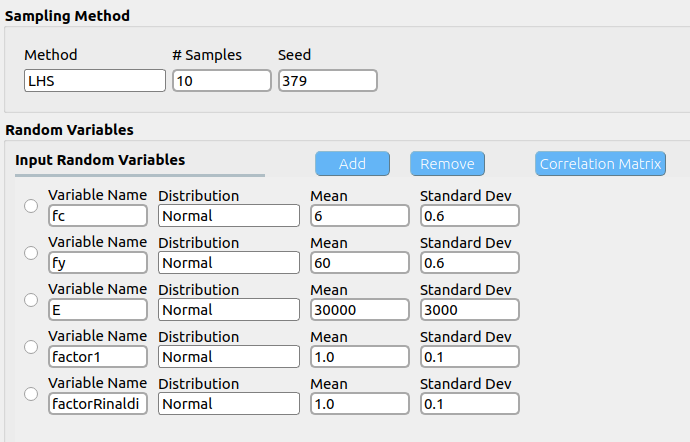
\includegraphics[width=0.8\textwidth]
    {usage/figures/uq1.png} }
  \caption{Uncertainty Quantification input panel}
  \label{fig:uq_panel}
\end{figure}

\subsection{Sampling Methods}
In the \href{https://dakota.sandia.gov//sites/default/files/docs/6.9/html-ref/method-sampling.html}{sampling methods} the user selects the sampling 
method to use from the dropdown menu. Currently there are two options available: 
Monte Carlo and Latin Hypercube Sampling (LHS). Depending on the option selected, the user must specifies the number of samples and the seed. The number of samples specifies the number of simulations to be performed. Providing a random seed allows the user to reproduce the same set of samples from the random variables multiple times.

\subsection{Random Variables}
The Random Variable panel allows the user to characterize the random
variables. Each random variable has a name and a distribution. The
distribution is selected from the drop-down menu. By changing the
distribution type, the parameters required to define the distribution
change. The following distributions are available (clicking on a link will take you to the Dakota manual that provides theoretical background and explains the requested parameters for each distribution):
\begin{enumerate}
\item \href{https://dakota.sandia.gov//sites/default/files/docs/6.9/html-ref/variables-normal_uncertain.html}{Normal}
\item \href{https://dakota.sandia.gov//sites/default/files/docs/6.9/html-ref/variables-lognormal_uncertain.html}{Lognormal}
\item \href{https://dakota.sandia.gov//sites/default/files/docs/6.9/html-ref/variables-beta_uncertain.html}{Beta}
\item \href{https://dakota.sandia.gov//sites/default/files/docs/6.9/html-ref/variables-uniform_uncertain.html}{Uniform}
\item \href{https://dakota.sandia.gov//sites/default/files/docs/6.9/html-ref/variables-weibull_uncertain.html}{Weibull}
\item \href{https://dakota.sandia.gov//sites/default/files/docs/6.9/html-ref/variables-gumbel_uncertain.html}{Gumbel}
\end{enumerate} 

As with other panels, the random variables can be added or
removed. Care must be taken by the user in ensuring that if the user
removes random variables from this panel that they also remove them
from the other input widgets. Failing to do so may result in the
program failing to complete.
